\documentclass{sigchi}

% Use this command to override the default ACM copyright statement (e.g. for preprints). 
% Consult the conference website for the camera-ready copyright statement.
\toappear{
Second draft
% Submitted for review.
}

% Arabic page numbers for submission. 
% Remove this line to eliminate page numbers for the camera ready copy
\pagenumbering{arabic}
% Load basic packages
\usepackage{balance}  % to better equalize the last page
%\usepackage{graphics} % for EPS, load graphicx instead
\usepackage{graphicx}
\usepackage{times}    % comment if you want LaTeX's default font
\usepackage{url}      % llt: nicely formatted URLs



% llt: Define a global style for URLs, rather that the default one
\makeatletter
\def\url@leostyle{%
  \@ifundefined{selectfont}{\def\UrlFont{\sf}}{\def\UrlFont{\small\bf\ttfamily}}}
\makeatother
\urlstyle{leo}


% To make various LaTeX processors do the right thing with page size.
\def\pprw{8.5in}
\def\pprh{11in}
\special{papersize=\pprw,\pprh}
\setlength{\paperwidth}{\pprw}
\setlength{\paperheight}{\pprh}
\setlength{\pdfpagewidth}{\pprw}
\setlength{\pdfpageheight}{\pprh}

% Make sure hyperref comes last of your loaded packages, 
% to give it a fighting chance of not being over-written, 
% since its job is to redefine many LaTeX commands.
\usepackage[pdftex]{hyperref}
\hypersetup{
pdftitle={User Modeling in Exploratory Search},
pdfauthor={LaTeX},
pdfkeywords={SIGCHI, proceedings, archival format},
bookmarksnumbered,
pdfstartview={FitH},
colorlinks,
citecolor=black,
filecolor=black,
linkcolor=black,
urlcolor=black,
breaklinks=true,
}

\DeclareGraphicsExtensions{.pdf,.png,.jpg}

% create a shortcut to typeset table headings
\newcommand\tabhead[1]{\small\textbf{#1}}


% End of preamble. Here it comes the document.
\begin{document}

\title{Supporting Exploratory Search in User Interface}

\def\tktl{Department of Computer Science\\University of Helsinki}
\def\tktladdr{P.O. Box 68 (Gustaf H\"allstr\"omin katu 2b)\\
FI-00014 UNIVERSITY OF HELSINKI\\
FINLAND}

\numberofauthors{2}
\author{
  \alignauthor Ilkka Kiistala\\
    \affaddr{\tktl}\\
    % \affaddr{\tktladdr}\\
    \email{ilkka.kiistala@helsinki.fi}
  \alignauthor Tuire Peurala\\
    \affaddr{\tktl}\\
    % \affaddr{\tktladdr}\\
    \email{tuire.peurala@helsinki.fi}
}

\maketitle

\begin{abstract}
Here we'll describe the content of our essay.
\end{abstract}

\keywords{
Exploratory Search; Information Retrieval; User Modeling.
}

\category{H.5.m.}{Information Interfaces and Presentation (e.g. HCI)}{Miscellaneous}


\terms{
Human Factors; Design; Measurement. 
}

\section{Introduction}
In this literature review we introduce the problem of exploratory search and some solutions for the problem. We cover three techniques that help the user in succeeding in his exploratory search task efficiently.
We explain what exploratory search is and what distinguishes it from other information retrieval tasks. 

To build a good system where machine and a human cooperate to perform a task it is important to take into account some significant characteristics of people \cite{rich99}. User model is built of these characteristics and traditionally it has been a model of a typical user \cite{rich99}. 

In reality often the users vary so much that a traditional user model is insufficient and there is a need for a user model of an individual.

Define ES

\cite{van08}: 
In order to accomodate to differing needs of users or usergroups over time, a system may use one of three basic approaches. System is called adaptive if it alters it structure, functionality or interface on the basis of a user model generated from \textit{implicit} user input. Adaptable systems use \textit{explicit user input} and need user's active participation. Personalized system is a hybrid of the two aforementioned.

In the following chapter we introduce basic concepts, solutions and systems that we found exploring the literature. 
In the Discussion chapter we summarize our findings and point out what is missing and what we expect from future research. 
The Conclusion chapter summarizes our findings.


\section{Literature review}
\label{sec:litreview}

(User Modeling) \cite{rich99}, \cite{fischer01}

\subsection{Exploratory Search}
(Ilkka)

Introduction to exploratory search.
\cite{march06}, \cite{white09}, \cite{tvaro11}

%% Palstan leveys tuntuu olevan n. 245pt

%\begin{figure}[p]
%\centering
%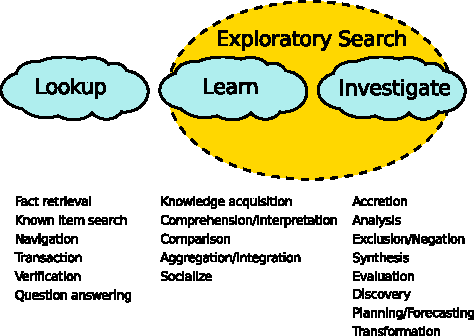
\includegraphics[bb=0 0 228 162]{clouds}
%\caption{Three clouds}
%\label{fig:clouds}
%\end{figure}

The user interface of an exploratory search system should be designed to fulfill the needs of most of its users. More information on what works and doesn't work can usually be collected from system evaluations.

However, evaluating exploratory search systems is difficult, because users have different starting positions. Their knowledge of the domain varies, they are interested in different aspects of the topic and they have previously encountered different information. \cite{kules08}

Exploratory search tasks can be characterized as either learning oriented or investigative  and they have common aspects like uncertainty, ambiguity and discovery distinguishing them from look-up oriented tasks \cite{kules09}.


\subsection{User Modeling}
(Tuire)

In the first ten years of Human-Computer interaction history the focus of research was in user interfaces and particularly the possibilities and design criteria of graphical user interfaces \cite{fischer01}. Later the focus has moved toward more broadly improving the way people use computers for example to work, think, communicate and learn \cite{fischer01}. To build a good system where computer and a human cooperate to perform a task it is important to take into account some significant characteristics of people \cite{rich99}. User models are built of these characteristics and are used to adapt the system toward the user. We define user models in this literature review as "models that systems have of users that reside inside a computational environment" \cite{fischer01}.

A central objective of user modeling is to address the problem that system will be unable to interact with users cooperatively unless they have some means of finding out what the user really knows and does \cite{fischer01}. To find out this there are two communication channels the explicit user input and the implicit information that is gathered without any effort from the users. The data gathered by these means is then used to improve the interaction with the system with the background knowledge of the problem domain, communication processes and the user agents involved (see Figure \ref{know_hci}).

\begin{figure}[htp] % t=top, h=here, b=bottom, p=separate page, !=place even if ugly
\caption{Knowledge-based HCI \protect\cite{fischer01}.}   \label{know_hci}
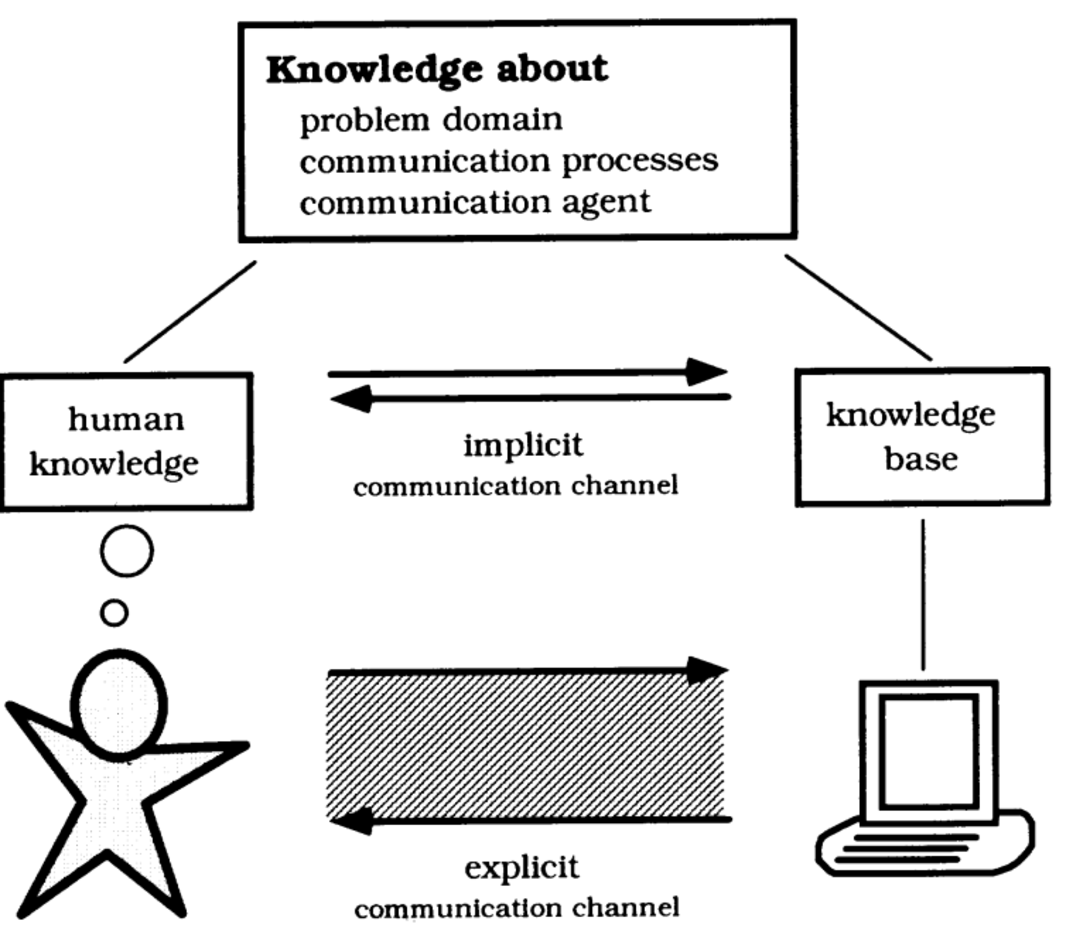
\includegraphics[scale=0.45]{figures/knowledge_hci.pdf} 
\end{figure}

In order to accomodate to differing needs of users or usergroups over time, a system may use one of three basic approaches \cite{van08}. System is called \textit{adaptive} if it alters it structure, functionality or interface on the basis of a user model generated from \textit{implicit} user input. \textit{Adaptable} systems use \textit{explicit} user input and need user's active participation. \textit{Personalized system} is a hybrid of the two aforementioned. In personalized systems the output or appearance differs for every user or user group in every context \cite{van08}. The adapted output has the potential to be of great benefit for users; it is geared towards the user's preferences, behaviour or needs and it can make interaction easier and a lot more fruitful. A lifecycle of a computational system cannot anymore be divided to the design time and use time as the behaviour of system can adapt to contextual information like the user goals only known at the use time. The differentiation between the design time and the use time of the system gets blurred with user modeling and the use time becomes design time \cite{fischer01}.

The different types of user models can be mapped as a three dimensional space where the axes are: single model vs. collection of models, explicitly specified models vs. models inferred by the system on the basis of user behaviour and long-term vs. short-term user models \cite{rich99}. The user model classification map is depicted in Figure \ref{dim_UM}. and the three dichotomies are explained further in this chapter. 

\begin{figure}[htp] % t=top, h=here, b=bottom, p=separate page, !=place even if ugly
\caption{The dimensions of user modeling.} \label{dim_UM}
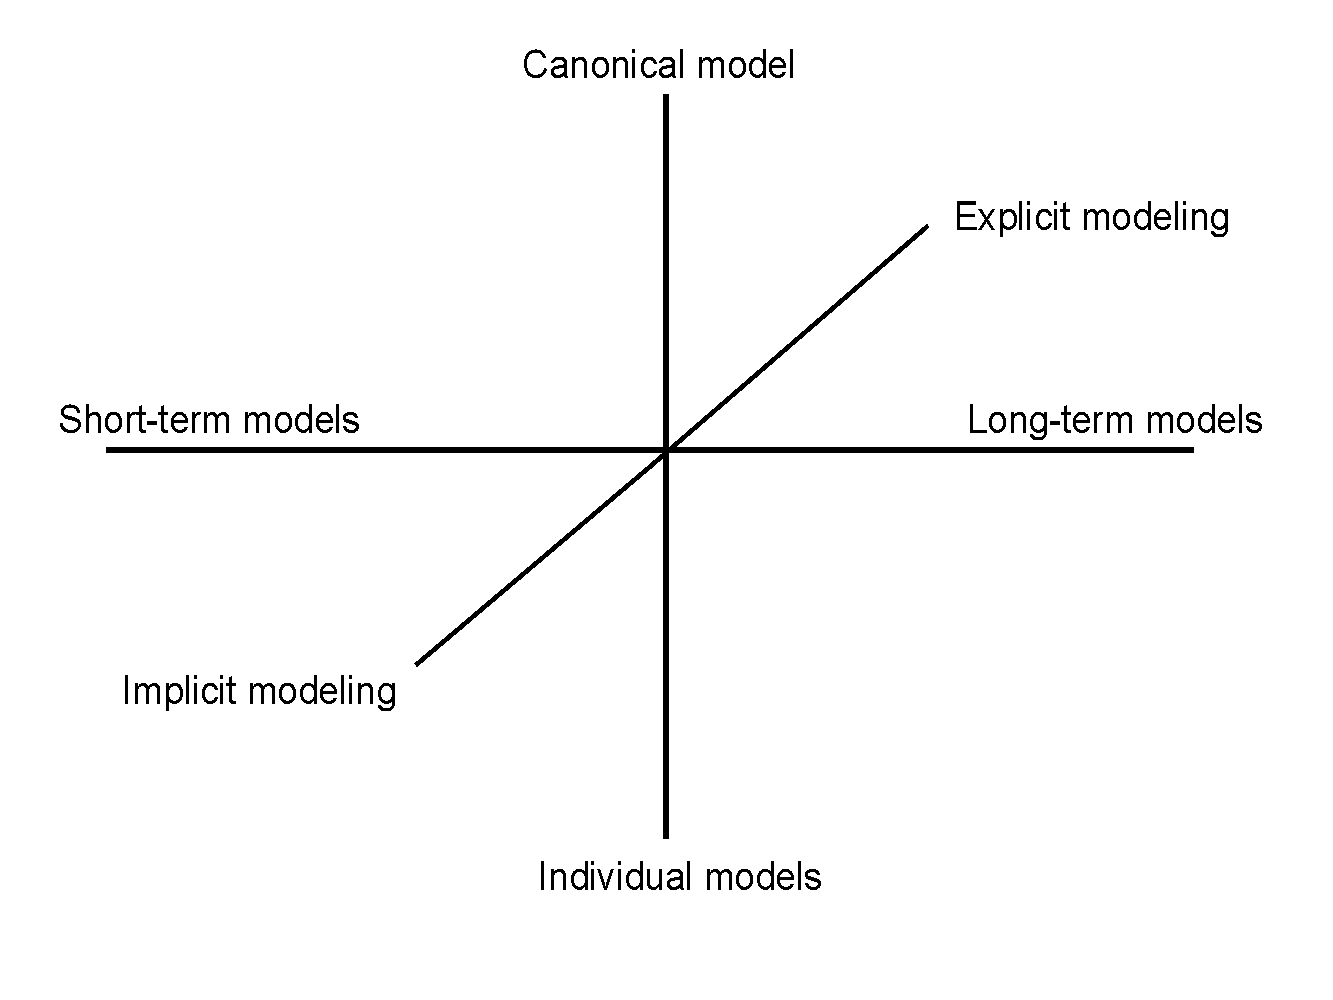
\includegraphics[scale=0.4]{figures/dimensions_UM.pdf} 
\end{figure}

The \textit{single model vs. collection of models} polarity \cite{rich99} has on it's other end the single model of single user. The modeled single user is called the canonical user and is actually not a real person at all but a modeled stereotypical user of the system. Traditional user models have been constructed by collecting data on an average user on various tasks and environments \cite{rich99}. An example of a canonical user model is Fitt's law that suggests that the speed on which the user operates the machine can be increased by increasing the size of targets the user must hit. The major weakness of these kind of models is that they assume that all the users constitute a homogenous set. In most cases for the majority of users the system is better adapted to them that would be without any adaptation, but it isn't likely the best system that could be produced \cite{rich99}. In the other end of this dichotomy is the collection of models of individual users. These users are real and the facts to build the individual model are gathered usually from the interaction of the user with the system. When choosing whether to use a canonical or individual user models one should think if the canonical model is sufficient or is the user community too heterogenous for it to be useful enough \cite{rich99}. The decision on this axis influences the other aspects of user modeling. If one user model is used then it has to be designed only once and the system doesn't have to prepare for incorrect or conflicting user model information as the case is on the latter option. 

The way how the user model is specified forms the second dichotomy mapping the user modeling techniques; \textit{explicit vs. implicit models} \cite{rich99}. On the explicit side the model is specified explicitly either by the system designer or by the users themselves. User model may be formed by letting the user modify the system but this leaves a lot on the hand of the user and fits badly to systems that expect to have lot of users that use the system only once or twice. Explicit user modeling can be done also by asking questions directly from the users but one problem with this is that users can't always answer on what the system needs to know. On the other end of the axis models are formed more subtly, they are inferred by the system only on the basis of user's behaviour. Implicit user models are built by gathering information of the user when the user interacts with the system. When constructing the user model implicitly the system must have some way of distinguishing incorrect information and resolving conflicts between gathered information.

In order to adapt soundly to the user the system must have wide variety of information about the user. The information might be ranging from short-term facts like the last query the user performed to more long-term facts like the level of mathematical sophistication of the user. This forms the third dichotomy: \textit{long-term vs, short term user models} \cite{rich99}. Long-term models can be built in the course of series of interactions between the system and the user. Long-term model could be built for example in a bookstore application where information of the user's purchases might be gathered to to recommend books of certain genre for the user. Short-term user model could be used in a search application. The model would be built by gathering recent queries to form a model of the user's search goal. Short-term user model is needed to respond to a situation where a user would need different search results when searching with keyword “Java” after searching information on programming or after the user has been searching beaches in Indonesia. There are also other differences in user models besides these introduced three dichotomies. Example of these differences is the model lifecycle; in a system where there is only a single model it can be permanently embedded with the system but in the case where there are models for each individual user the model is built on the fly. This and many other differences follow from the aforementioned three axes and are not distinguished as categorizing user models \cite{rich99}. 



 

(oli: Personalization)
Individualization of user models, Adaptive/Adaptable User Interfaces, intelligent user interfaces
\cite{bunt04}, \cite{findlater04}, \cite{brusi96}

\cite{van08}: The evaluation of a personalized system is problematic because it is unclear if the results gathered from a few individuals who all used system personalized for them can be generalized to entire population of users.

Including adaptive elements in the user interface might increase the workload of the user. When users had two alternative interfaces to a menu, an adapted one and a full one, there was cognitive overhead in 1) having to decide which features to include in the personalized interface and 2) having to figure out a menu item was missing and that changing to the full interface would make it appear in the menu again \cite{bunt04}.

(Kun tiedetään käyttäjästä jotain... jatketaan Solutions-kohtaan)

Search systems have evolved from simple "query to results" paradigm to a clever system that utilizes the user model to provide the user with better search results. Instead of providing results based on solely the search word, the search system can extend the search beyond the search word and, for example, include some synonyms in the query. Or the search system might recognize a common typo in the search query and replace the misspelled word with the correct one. The system might ask the user to rate the result of the search and then change accordingly. (faceted search jonnekin) In the following subsections we cover three different solutions that support exploratory search: faceted search, relevance feedback and query expansion.

\subsection{Faceted search}

Information seekers often express a desire for a user interface that organizes search results into meaningful groups, in order to help make sense of the results and to help decide what to do next \cite{hearst06}. There two ways of grouping search results; clustering and hierarchical faceted categories. Clustering is grouping of items based on some similarity and is fully automated process. It is good for clarifying a vague query but the clustering algorithms aren't yet perfect and the clustering can be unpredicted \cite{hearst06}. Category system is a set of labels that are organized to mirror the domain. Hierarchical faceted categories are a set of hierarchical categories that each represent a different dimension. Categories are usually created manually but can be partly automated. 

\cite{kules09}:The writers had done a user experiment to find out what  the searchers are  looking at in a faceted search UI. The test participants were  university students and the system of interest was a library system. As a result  of the eyetracker test the writers found out that participants looked a lot at the facets and  47,4\% of the  eye movement  was between facets, breadcrums summarising the selected facets and the result list. In an interview the participants told they used facets to help organize their view on the topic domain and select sub-topics for further investigation. Of these results the researchers deduced that the facets played an important role in the exploratory search process. 
The article summarizes related study on faceted search and exploratory search and has many interesting leads on articles for our essay topic.

Exploratory search is a complex information seeking task and to support this it has become accepted to use faceted search or categorized overviews \cite{kules09}. Structured metadata is used to provide the user with an overview of the results and clickable categories. With this UI approach the user doesn't have to reformulate the query to narrow and browse the results. Faceted search is used in practice in library catalogs, web search, online shopping and other domains \cite{kules09}. Faceted search enables the user to change fluidly between search and browsing and searchers with partially defined or changing information needs can use the overview to understand the knowledge domain and refine their needs. It has been shown that when using faceted search the users explored their results more broadly than without facets and felt more organized about their searches. Still though the faceted search interfaces make the search more efficient the subjects don't always prefer it \cite{kules09}. 

\cite{shen05}The writers have developed a client-side web search agent to work on top of google and they claim it improves the accuracy of the results. In information retrieval the user model/information need is “traditionally” (2005) constructed only by the query keywords and improved by relevance feedback where the user is asked to implicitly specify which of the results are relevant. As the users are usually reluctant in doing this, the writers have developed an implicit model for improving the search user model. Usually user models are long-lived but this model is concentrated on short-term context. The search agent tries to respond to a situation where a user would need different results for searching with keyword “Java” after searching programming stuff or after the user has been searching beaches in Indonesia. Two challenges for information retrieval systems are identified: 1. different users may use the exactly same keywords to look for different things and 2. the information needs of a user may change over time. In their search agent the writers gather information from two sources; the previous query keywords and the viewed document summaries. The system responds immediately to each user action with a system action and the user doesn’t have to actively take part on adapting the search result to be more relevant.

- System examples
\subsection{Relevance feedback}
(also User Modeling) 

The goal of user modeling for a search system is to model a user's information need. The obvious source of information is the query. But as the queries tend to be quite short, especially when using a mobile device, the search words may not be a very accurate source of information for the user's information need. Much more data is available if user is given the opportunity to give feedback on the search results. 

It is a way to teach the system about user’s preferences. The user uses the explicit communications channel to give the system some information about the context. In practise, when a search result is shown to the user the system provides a way for user to respond if the result was sufficient or not. The user might rate the result, for example with stars to point out how successful the system was in finding the results for the user’s query. However, relevance feedback requires a system that incorporates and utilizes the given feedback and of course, it requires the user to use time and energy to evaluate the search result and how the result fills the need of the information retrieval task at hand. The extra effort has been shown to be too great a burden to users and thus relevance feedback is considered a scarce source for user model data.

This \emph{relevance feedback} has been found to improve retrieval accuracy \cite{salton90}. This, however, requires extra effort from the users and users are reluctant to make extra effort \cite{kelly03}. As \cite{shen05} shows, user action data can be used to improve the search results without the extra effort. They collected all the actions the user did and used them to update the user model. This user model was used in customizing the ranking which the results were based on.
- System examples
\subsection{Query expansion}
- System examples

\subsection{Query Term Suggestion}

Such search interfaces have appeared that suggest query terms dynamically, as the user enters them. In some of the systems the term suggestions appear before the searcher has seen any retrieval results, and in others, the system dynamically shows documents that match the characters typed so far, adjusting the results list as more characters are typed. Dynamic query term suggestions (sometimes referred to as auto-suggest, autosuggest, or search-as-you-type) are becoming a widely used solution between requiring the user to know exactly how to spell the query terms and to think of relevant and connected terms overall. [Hearst]

Some dynamic term suggestion systems show only query suggestions whose prefix matches what has been typed so far. Figure X shows an example from Google’s dynamic query suggestions interface, which shows queries where the prefix matches some words used in previously used queries – in this example, “query sug” matches “query suggestion”. Dynamic query suggestions are not restricted to matching the prefix of the query alone.  (joku esimerkki) . 

\begin{figure}[htp] % t=top, h=here, b=bottom, p=separate page, !=place even if ugly
\caption{One view of dynamic query term suggestions. An example from Google in which the prefix of a word in the query is matched against past queries. \protect.}   \label{querysuggestion}
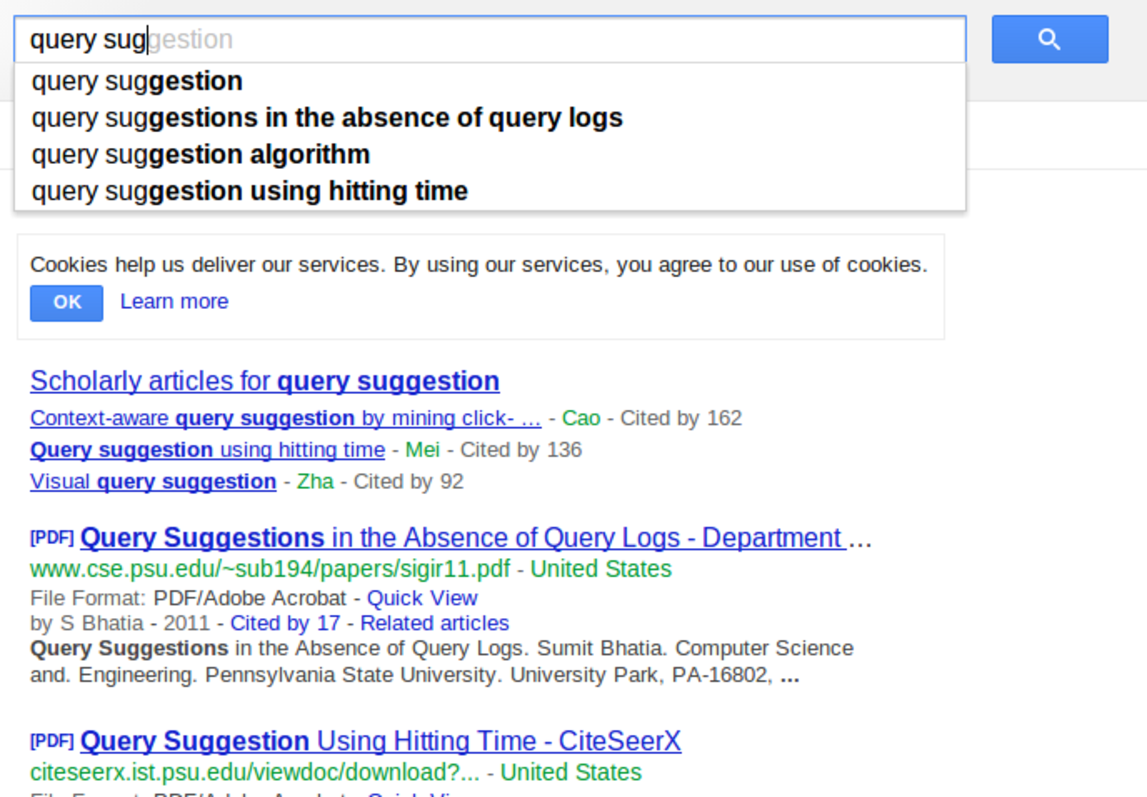
\includegraphics[scale=0.41]{figures/dynamicQueryTermSuggestion2.pdf} 
\end{figure}


\section{Discussion}
In the Discussion chapter we summarize our findings and point out what is missing and what we expect from future research. 

Future challenges for user modeling : payoff, user modeling vs. task modeling, wrong/outdated info, adequacy of models, larger context, user's loss of control, privacy concerns \cite{fischer01}.

\section{Conclusion}
Goal, solution summary

Our goal was to explore the field of Exploratory Search and User Modeling. We found several articles that have some contribution to the topic.

Summary of results and their reliability 

We found that:
- Usage
- Success
- Failures

How much is it used in the real world, really?

Research impact
- What has the research brought into software development?

\nocite{*} %tämä listaa kaikki viitteet luetteloon vaikka niitä ei olisi vielä viitattu

% Balancing columns in a ref list is a bit of a pain because you
% either use a hack like flushend or balance, or manually insert
% a column break.  http://www.tex.ac.uk/cgi-bin/texfaq2html?label=balance
% multicols doesn't work because we're already in two-column mode,
% and flushend isn't awesome, so I choose balance.  See this
% for more info: http://cs.brown.edu/system/software/latex/doc/balance.pdf
%
% Note that in a perfect world balance wants to be in the first
% column of the last page.
%
% If balance doesn't work for you, you can remove that and
% hard-code a column break into the bbl file right before you
% submit:
%
% http://stackoverflow.com/questions/2149854/how-to-manually-equalize-columns-
% in-an-ieee-paper-if-using-bibtex
%
% Or, just remove \balance and give up on balancing the last page.
%
\balance

% If you want to use smaller typesetting for the reference list,
% uncomment the following line:
% \small
\bibliographystyle{acm-sigchi}
\bibliography{umines}
\end{document}
